\chapter{Einleitung}

Diese kleine Einleitung soll dem Nutzer helfen selbst die eigene Arbeit mit \LaTeX{} zu schreiben. Sie enth"alt Beispiele zu den wichtigsten Themen .

\blindtext

\section{Dokumentlgiederung}

Für diese Arbeit verwendet man folgende LaTeX-Kommados zur Strukturierung:

\begin{verbatim}
\chapter{Einleitung}
\section{Dokumentgliederung}
\subsection{}
\subsubsection{}
\end{verbatim}

Allerdings sollte man sich überlegen, ob man wirklich bis zur Stufe \verb|subsubsection| "Uberschriften benötigt.

\section{Illustrationen}

\blindtext

\blindtext

\subsection{Bilder und Abbildungen}

Auch in einer wissenschaftlichen Arbeit können Bilder und Abbildungen zur Veranschaulichung und zur Illustration sachlicher Inhalte integriert und einfügt werden. Für Fotografien und Bilder unterstützt PDF-\LaTeX{} direkt \verb|jpg| und \verb|png|. Ansonsten empfiehlt es sich, Vektorgrafiken zu verwenden und diese als \verb|pdf| zu speichern. Sollte ein Bild einmal von zu viel weißem Raum umgeben sein, kann man mit dem Werkzeug \verb|pdfcrop| das Bild automatisch zuschneiden.

\begin{figure}[ht]
\centering
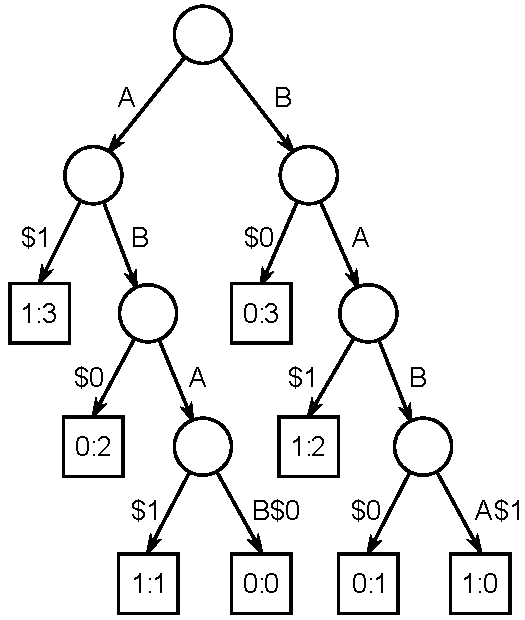
\includegraphics[width=.4\textwidth]{images/Suffix_tree_ABAB_BABA}
\caption{\label{fig:bild1}Beschreibung/Beschriftung des Bilds}
\end{figure}

Mit Hilfe eines Labels \verb|\label{fig:bild1}| kann man sich dann im fortlaufenden Text mittels eines Querverweises auf diese Grafik beziehen: \verb|\ref{fig:bild1}|. An der Stelle des ref-Kommandos platziert LaTeX die Nummer der Abbildung: \glq siehe Abbildung \ref{fig:bild1}\grq.


\subsection{Tabellen}
\label{sec:tabellen}

Seite \pageref{tab:beispieltabelle}, Abschnitt \ref{sec:tabellen}, enthält Beispieltabelle \ref{tab:beispieltabelle}. In vielen \LaTeX{}-Büchern finden sich gute Anleitungen zum Erstellen von Tabellen. Komplexere Tabellen können sinnvollerweise in Excel oder einer anderen Tabellenkalulation vorgefertigt und mit einem Umwandlungsprogramm oder -werkzeug in LaTeX-Quellcode konvertiert werden.

\begin{table}[h]
\begin{center}
\begin{tabular}{|lll|}
    \hline
	A & B & C \\
	\hline
	x & x & x \\
	x & x & x \\
	\hline
\end{tabular}
\end{center}
\caption{Eine kleine Beispieltabelle}
\label{tab:beispieltabelle}
\end{table}


\subsection{Formeln}

Mathematische Formeln lassen sich in der Umgebung  \verb|math| erzeugen. Die Kurz- Schreibweise lautet \verb|\( a^2+b^2=c^2 \)|;  hierbei steht die Formel dann im laufenden Text: \( a^2+b^2=c^2 \). Die kürzeste Form ist mit zwei \verb|$| um die Formel, z.B.~so: Wasser ist H$_2$O. \verb|H$_2$O|

Mit der Schreibweise \verb|\[ y=x^2 \]| wird die Formel mittig in einer eigenen Zeile gesetzt, z.B.

\[y = x^2 \]

Formeln in der Umgebung \verb|equation| werden mittig in einer eigenen Zeile gesetzt und fortlaufend nummeriert:

\begin{equation}
x_{1,2} = \frac{-b\pm\sqrt{b^2-4ac}}{2a}
\label{mitternachtsformel}
\end{equation}
Wenn wir z.B.~über die beliebte Mitternachtsformel (Gleichung \ref{mitternachtsformel}) Details im umliegenden Text schreiben wollen, lässt sich diese wie ein Bild oder eine Tabelle referenzieren, sofern man ihr ein Label zugewiesen hat..


\subsection{Programmier-Code}

Mehrzeiliger Programmier- und Quellcode kann mit \verb|verbatim| in einer Umgebung gesetzt werden:

\begin{verbatim}
  Dieser Text steht in einer verbatim-Umgebung und wird daher
  in Schreibmaschinenschrift geschrieben.
  LaTeX-Kommandos, z.B. \includegraphics[width=.6\textwidth]{bild.jpg}
  werden nicht interpretiert, sondern "verbatim" ausgegeben.
\end{verbatim}

Schöner und professioneller lässt sich Programmier-Code mit dem \verb|listings|-Paket, eingeben, formatieren und ausgeben. Dazu kann man in der Präambel die Sprache angeben, in der die Quellcodes geschrieben sind.

\begin{lstlisting}
public class Hello {
    public static void main(String[] args) {
        System.out.println("Hello World");
    }
}
\end{lstlisting}

Innerhalb einer Zeile gibt man Wörter am Besten als \verb|\verb##| an, dabei erwartet \LaTeX{} zweimal das gleiche Zeichen als Begrenzer. Im Beispiel ist dies die Raute \verb|#|, man kann aber auch jedes andere Zeichen nehmen, z.B. das Plus $+$.



\section{Text}

Textteile können bei Bedarf mit dem Befehl \verb|\emph{}| \emph{hervorgehoben} werden. Falls in einem Satz ein Punkt vorkommt, macht man danach kein Leerzeichen sondern eine Tilde (\verb|z.~B.~so!|), denn dann fügt \LaTeX{} den korrekten Abstand ein, z.~B.~so!


In der Präambel der vorliegenden tex-Datei gibt es den Befehl \verb|hypenation|, der zur Silbentrennung da ist. \LaTeX{} verfügt zwar über  eine eingebaute Silbentrennung, die jedoch bei manchen Wörtern falsch trennt. Damit diese Wörter korrekt getrennt werden, gibt man sie dann mit dem Befehl in der Präambel an\footnote{Das Wort \emph{Silbentrennung} ist hier das Beispiel}.

Fußnoten werden mit dem Befehl \verb|footnote| mitten in den fortlaufenden Text eingefügt. \footnote{Wie man schon im vorherigen Absatz sehen konnte.}

In wissenschaftlichen Arbeiten muss man des öfteren andere Arbeiten zitieren. Dazu nutzt man die Stiloptionen und Zitierbefehle des Pakets \verb+biblatex+, z.\,B.\,\verb|numeric| (=Standard-Stil) oder \verb|verbose| resp. \verb|\cite{name}| oder \verb|\autocite{name}|. In eckigen Klammern kann man noch die Seitenzahl angeben, falls notwendig. Der Name ist ein Schlüssel aus der Datei \verb|bibliography.bib|. Falls einmal ein Werk nur indirekt zu einem Teil der Arbeit beigetragen hat, kann man es auch mit \verb|nocite| angeben, dann landet es in der Literaturliste, ohne dass es im Text ausdrücklich zitert wird.


\subsection{Weiterführendes}

Zum Schluss sei auf die Vielzahl an Büchern zu \LaTeX{} verwiesen. In jeder Bibliothek wird sich eine Einführung finden, in der dann weitere Themen wie mathematische Formeln, Aufbau von Briefen und viele nützliche Erweiterungen besprochen werden.

